\documentclass[11pt,a4paper]{article}

\usepackage[margin=1in]{geometry}
\usepackage{amsmath,amssymb}
\usepackage{booktabs}
\usepackage{array}
\usepackage[T1]{fontenc}
\usepackage{graphicx}
\usepackage{tikz}
\usepackage{enumitem}
\usepackage{url}
\usepackage[colorlinks=true,linkcolor=blue,urlcolor=blue]{hyperref}
\usetikzlibrary{positioning,arrows.meta}

\newcommand{\TBD}{\textbf{TBD}}

\begin{document}

\title{\textbf{Real-Time Surveillance Event Detection Using CNN-Based Multiclass and Binary Classification}}\
\author{Project documentation}
\date{\today}
\maketitle

\begin{abstract}
This project implements a camera-based surveillance event detection prototype in which a Flask backend streams frames from a local camera and runs image classification using TensorFlow/Keras CNN models. The current repository contains one multiclass model for the classes \emph{normal}, \emph{fire}, \emph{accident}, and \emph{violence}, together with three independently trained binary models for \emph{fire vs normal}, \emph{violence vs normal}, and \emph{accident vs normal}. The frontend presents the multiclass probabilities, binary probabilities, and a comparison between the two decisions. The implementation is image-based and is therefore limited to single-frame classification; explicit temporal modeling is not implemented in the current codebase. The dataset structure, preprocessing pipeline, model architecture, and training scripts are implemented and documented here, while final reported evaluation metrics are intentionally left as \TBD or preliminary results because the repository does not include a finalized, archived held-out evaluation report.
\end{abstract}

\section{Introduction}
\subsection{Background}
Modern surveillance systems often monitor large volumes of video feeds and require automated detection of abnormal or hazardous events. Many practical deployments rely on computer vision methods for scene understanding, event classification, and alerting. Within this context, deep learning approaches based on convolutional neural networks (CNNs) have become a common choice for image classification because they can learn hierarchical visual features directly from data. This project studies the application of CNN-based classification to a small surveillance-event taxonomy composed of four classes: normal, fire, accident, and violence. In the current implementation, the system is limited to static frame analysis and does not explicitly model temporal dependencies across frames.

\subsection{Motivation}
The repository is motivated by a practical comparative question: for the same surveillance-event classification task, should the system use one multiclass CNN or several independent binary CNNs? Both alternatives are implemented and compared in the frontend. This design allows a direct visual comparison of class probabilities and event decisions under the same input frame, which is useful for an experimental study of false positives, false negatives, and class confusion. The practical motivation is educational and exploratory: to compare two CNN-based classification designs in a lightweight image-processing pipeline rather than to claim a production-ready system.

\subsection{Problem Statement}
The primary problem addressed by the project is to classify a surveillance frame into one of four event categories while also comparing the outcome of a multiclass classifier against three binary classifiers. The dataset and the current model setup are small-scale and image-based, so the system is better characterized as a prototype for comparison and experimentation than as a complete, deployable emergency monitoring platform. The repository also highlights limitations such as uneven class coverage, possible consecutive-frame similarity in certain classes, and the absence of a clearly separated held-out test set.

\subsection{Objectives}
The objectives of the implemented project are as follows:
\begin{itemize}[leftmargin=1.5em]
    \item To build a simple Flask-based surveillance application that streams frames from a camera.
    \item To preprocess frames in a deterministic image pipeline compatible with trained CNNs.
    \item To train and load a 4-class CNN for \emph{normal}, \emph{fire}, \emph{accident}, and \emph{violence} classification.
    \item To train and load three independent binary CNNs for event detection against a normal class.
    \item To compare multiclass and binary decisions in a single inference pass.
    \item To document the implementation, limitations, and planned refinement strategy.
\end{itemize}

\subsection{Scope}
The current repository scope is limited to a local prototype. It includes camera access via OpenCV, Flask endpoints for live streaming and detection, TensorFlow/Keras image models, and a static frontend dashboard. The system does not include large-scale training pipelines, cloud deployment, alert communication infrastructure, or explicit temporal tracking. The project therefore sits in the category of a small-scale academic prototype rather than a finished commercial surveillance platform.

\subsection{Contributions}
The current project contributes a comparison-oriented implementation in which:
\begin{enumerate}[leftmargin=1.5em]
    \item A single-frame multiclass CNN classifier is implemented.
    \item Three separate binary CNN classifiers are implemented for event-specific detection.
    \item A frontend dashboard compares the outputs of both approaches on the same frame.
    \item The repository documents the training and inference pipeline and the dataset folder structure.
    \item The project explicitly treats the comparison as an experimental study with known dataset and evaluation caveats.
\end{enumerate}

\section{Literature Review}
The literature relevant to this project spans multiple areas: deep learning for image classification, surveillance video analysis, and event-specific classification tasks such as fire, violence, and accident detection. The current codebase is not built around a specific published architecture but follows a standard CNN design and stores trained Keras models for later inference.

\subsection{Computer Vision for Surveillance}
Surveillance video analytics has long been studied as a task in which a system must detect abnormal or hazardous events from visual input under varying lighting, occlusion, and scene complexity. Classical approaches relied on handcrafted motion, texture, and background-subtraction features, while modern systems increasingly use deep learning pipelines to learn discriminative representations directly from images or video clips. The main challenge is not only event recognition but also robustness against false alarms in everyday scenes and the need to minimize missed detections in hazardous conditions. This project follows the image-based CNN direction, but it does not yet implement explicit temporal modeling or tracking.

\subsection{CNNs for Image Classification}
A foundational influence on modern CNN-based computer vision is the ImageNet classification work by Krizhevsky, Sutskever, and Hinton \cite{krizhevsky2012}, which demonstrated that deep convolutional architectures trained end-to-end can substantially improve image classification performance. Subsequent work by Simonyan and Zisserman \cite{simonyan2015} showed that deeper CNN architectures can further improve representational power, and He et al. \cite{he2016} introduced residual learning to ease optimization in very deep networks. These papers are relevant because the implemented CNN architecture in this project follows the standard deep-learning pipeline of stacked convolutional layers, pooling, flattening, and fully connected classification heads, but on a much smaller task and dataset than ImageNet-scale benchmarks.

\subsection{Deep Learning for Fire Detection}
Fire detection is a common surveillance task because it often requires rapid identification of a hazard in images or video streams. Deep learning systems for fire detection typically model the problem as a binary classification or detection task using visual cues such as smoke, flame color, intensity, and scene context. The current implementation follows a simplified binary formulation in which a dedicated fire-vs-normal CNN is trained and evaluated separately from the multiclass model. This is consistent with the practical need to handle event-specific classifications in a small prototype, but it does not represent a full fire-detection system with temporal reasoning, smoke modeling, or multi-camera coordination.

\subsection{Deep Learning for Violence Detection}
Violence detection in surveillance contexts is a difficult problem because it requires recognizing aggressive or threatening human activity from visual cues that can vary significantly across scene viewpoint, body pose, and context. Methods in the literature range from handcrafted motion features to modern spatiotemporal CNNs and action-recognition models. A useful conceptual connection is the action-recognition literature on temporal modeling, such as the work of Carreira and Zisserman on Kinetics-based action recognition \cite{carreira2017} and the temporal segment network work by Wang et al. \cite{wang2016}, which highlights the role of temporal information in recognizing actions and interactions. The current repository does not implement such temporal modeling; instead, it performs per-frame classification.

\subsection{Deep Learning for Accident Detection}
Accident detection is often treated as an abnormal-event problem in road or surveillance scenes. Research in this area typically focuses on vehicle motion, collision patterns, unusual trajectories, and scene context in video streams. In a frame-level image classification setting, accident examples are usually represented by visual cues extracted from specific incident frames. The repository notes that the accident dataset contains consecutive or near-consecutive frames from video sequences, which introduces a dataset quality challenge for image-based learning. This observation is consistent with the broader difficulty of creating fair accident datasets without train/test contamination from temporally similar frames.

\subsection{Multiclass vs Binary Classification}
A multiclass formulation assigns one label among several event types, while binary classification trains a model to distinguish one event from a normal class. In theory, multiclass learning can capture cross-class relationships, whereas binary learning can isolate event-specific decision boundaries. For surveillance tasks with a small number of classes, both approaches are reasonable, but their practical behavior depends strongly on class balance, dataset quality, and the degree of similarity among classes. The current project intentionally compares these two formulations on the same image-based task with the same preprocessing pipeline and a single frontend comparison layer.

\subsection{Video/Temporal Information in Surveillance}
Many surveillance events are intrinsically temporal. Fire may spread over time, fights may evolve across consecutive frames, and accidents may involve motion and interaction patterns that cannot be fully captured by a single still image. The action-recognition literature has shown that temporal modeling can improve event recognition when motion information is important. The present repository does not implement temporal modeling, which is a limitation discussed in the current system limitations section. This is consistent with an image-level prototype rather than a complete video-understanding system.

\subsection{Research Gap / Motivation for the Proposed Comparison}
The main research question in this project is not a claim of a wholly new model but a practical comparison of two architecture choices on the same surveillance-event classification task: a single multiclass classifier versus three independent binary classifiers. This is relevant because false positives, false negatives, and class confusion can differ substantially between the two designs even when the training data and preprocessing are similar. The current repository is therefore best understood as an experimental comparison rather than as a novel algorithmic contribution.

\section{System Overview}
\subsection{Overall Architecture}
The implemented application is a lightweight web-based surveillance pipeline that combines a Flask backend, OpenCV frame capture, TensorFlow/Keras classifiers, and a JavaScript frontend. The architecture is shown in Figure~\ref{fig:overall-architecture}. In the current implementation, a camera stream produces frames in BGR format, the backend converts them to RGB for preprocessing, and the same frame is processed by both the multiclass model and the binary models. The outcomes are then merged into a comparison object and returned to the frontend for display.

\begin{figure}[h]
\centering
\begin{tikzpicture}[
  node distance=2.5cm and 2.5cm,
  box/.style={draw, rounded corners, align=center, minimum width=2.8cm, minimum height=1.1cm},
  arrow/.style={->, >=Stealth, thick}
]

\node[box](camera){Camera};
\node[box,right=of camera](backend){Flask backend};
\node[box,right=of backend](preprocess){Frame preprocessing};
\node[box,above right=of preprocess](multi){Multiclass CNN};
\node[box,below right=of preprocess](binary){Binary CNNs};
\node[box,right=of preprocess, xshift=5cm](frontend){Frontend comparison};

\draw[arrow] (camera) -- (backend);
\draw[arrow] (backend) -- (preprocess);
\draw[arrow] (preprocess) -- (multi);
\draw[arrow] (preprocess) -- (binary);
\draw[arrow] (multi) -- (frontend);
\draw[arrow] (binary) -- (frontend);

\end{tikzpicture}
\caption{Overall system architecture of the current prototype.}
\label{fig:overall-architecture}
\end{figure}

\subsection{Frontend}
The frontend is a static HTML/CSS/JavaScript interface stored in the \texttt{frontend/} directory. It includes a start/stop camera control and a video display area that receives a live MJPEG-like stream from the Flask backend. In the current dashboard, detection probabilities for each class are presented in both the multiclass and binary views, along with the final event label and an agreement indicator between the two models. The JavaScript polling logic fetches the result from the backend endpoint every second.

\subsection{Backend}
The backend consists of a Flask application with a blueprint-based route structure. The file \texttt{backend/app.py} creates the Flask app and registers the routes defined in \texttt{backend/routes.py}. The route structure includes:
\begin{itemize}[leftmargin=1.5em]
    \item \texttt{/} to serve the frontend entry page,
    \item \texttt{/start\_camera} and \texttt{/stop\_camera} to control a local OpenCV camera,
    \item \texttt{/video\_feed} to stream frames,
    \item \texttt{/detection} to return JSON detection results.
\end{itemize}
The actual camera logic and detection pipeline are placed in \texttt{backend/controllers.py}. This file uses \texttt{cv2.VideoCapture(0)} and updates a global frame buffer and detection result. A lightweight detection cadence is enforced by a one-second interval and a lock-based mechanism to avoid overlapping inference calls.

\subsection{Machine Learning Layer}
The machine learning layer resides in \texttt{ml/detection.py} and loads the trained Keras models from the \texttt{ml/trained\_models/} directory. The current repository contains the following trained files:
\begin{itemize}[leftmargin=1.5em]
    \item \texttt{surveillance\_model.keras}
    \item \texttt{binary\_fire\_model.keras}
    \item \texttt{binary\_violence\_model.keras}
    \item \texttt{binary\_accident\_model.keras}
\end{itemize}
All models are TensorFlow/Keras models. The multiclass model outputs four probabilities corresponding to normal, fire, accident, and violence, while each binary model outputs a single sigmoid probability for an event-vs-normal decision. The backend loads these models once and reuses them for repeated inference.

\subsection{Inference Pipeline}
The current inference path is single-frame based. Figure~\ref{fig:multiclass-pipeline} shows the multiclass flow, and Figure~\ref{fig:binary-pipeline} shows the event-specific flow. The process is:
\begin{enumerate}[leftmargin=1.5em]
    \item Capture a frame from the camera with OpenCV.
    \item Convert BGR to RGB.
    \item Resize to $128\times128$ and scale pixel values to $[0,1]$.
    \item Feed the processed array to the model.
    \item Compute class probabilities and the final event label.
    \item Compare this with the binary-model decision and return both results.
\end{enumerate}

\begin{figure}[h]
\centering
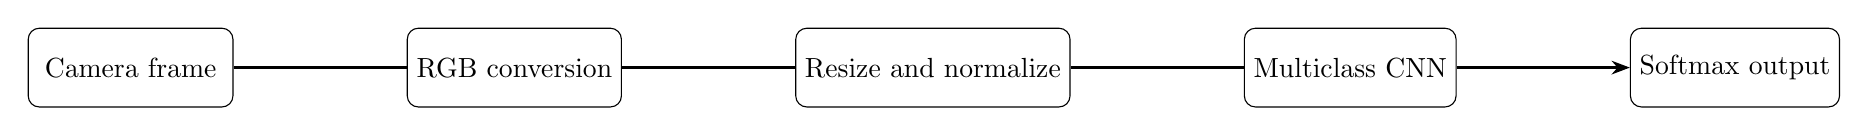
\begin{tikzpicture}[
  node distance=2.1cm and 2.2cm,
  box/.style={draw, rounded corners, align=center, minimum width=2.6cm, minimum height=1cm},
  arrow/.style={->, >=Stealth, thick}
]
\node[box](frame){Camera frame};
\node[box,right=of frame](rgb){RGB conversion};
\node[box,right=of rgb](prep){Resize and normalize};
\node[box,right=of prep](cnn){Multiclass CNN};
\node[box,right=of cnn](out){Softmax output};
\draw[arrow] (frame)--(rgb)--(prep)--(cnn)--(out);
\end{tikzpicture}
\caption{Current multiclass inference pipeline.}
\label{fig:multiclass-pipeline}
\end{figure}

\begin{figure}[h]
\centering
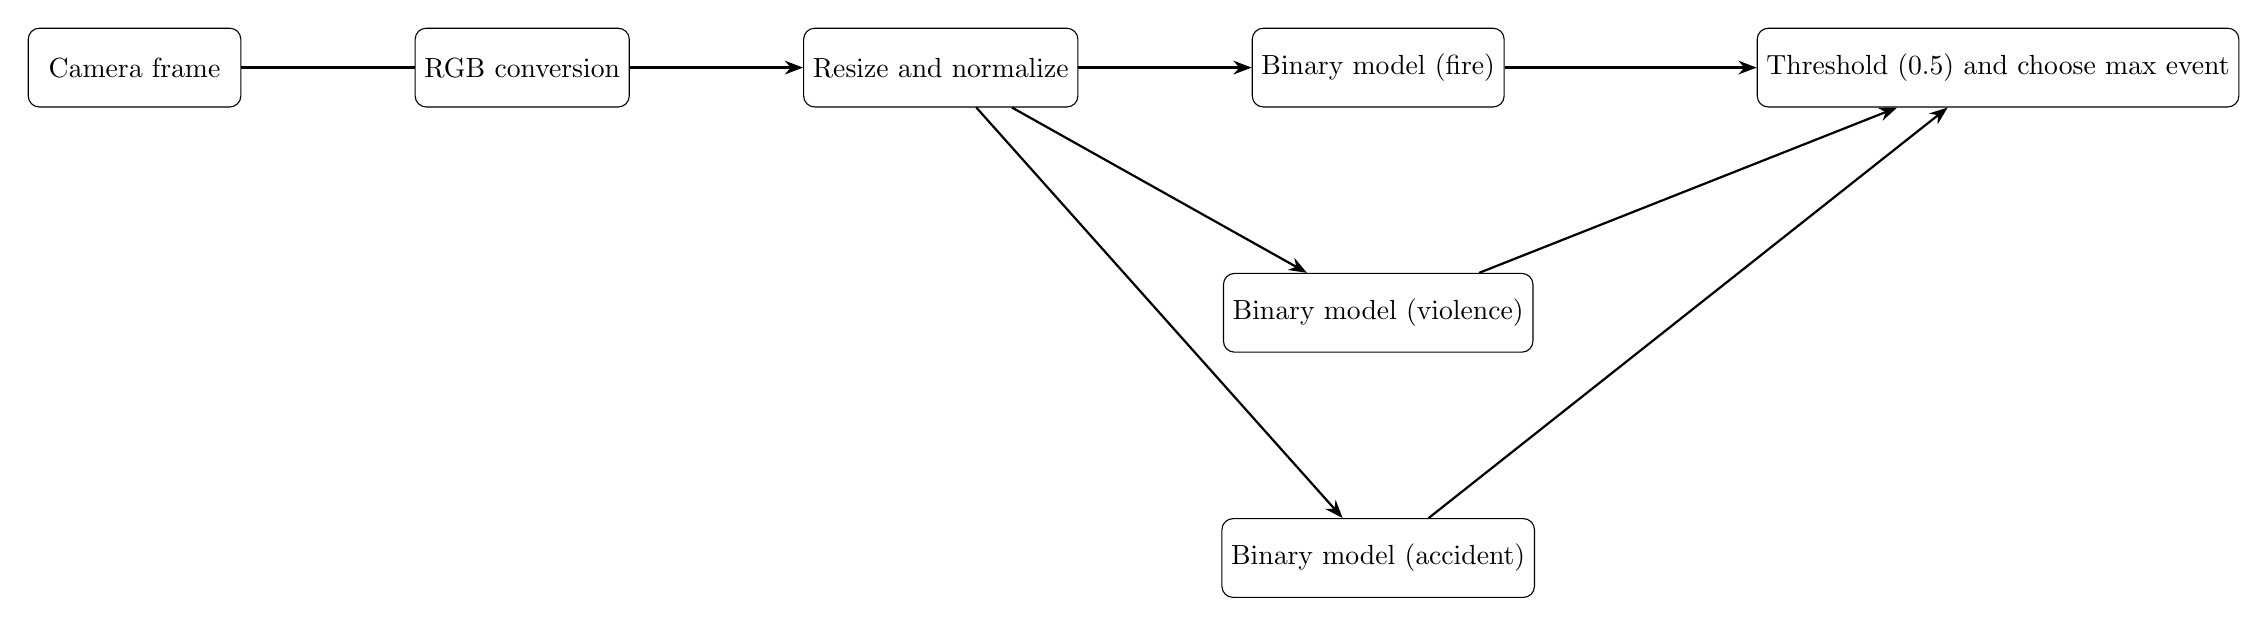
\begin{tikzpicture}[
  node distance=2.1cm and 2.2cm,
  box/.style={draw, rounded corners, align=center, minimum width=2.7cm, minimum height=1cm},
  arrow/.style={->, >=Stealth, thick}
]
\node[box](frame){Camera frame};
\node[box,right=of frame](rgb){RGB conversion};
\node[box,right=of rgb](prep){Resize and normalize};
\node[box,right=of prep](fire){Binary model (fire)};
\node[box,below=of fire](violence){Binary model (violence)};
\node[box,below=of violence](accident){Binary model (accident)};
\node[box,right=of fire, xshift=1.0cm](combine){Threshold $(0.5)$ and choose max event};
\draw[arrow] (frame)--(rgb)--(prep);
\draw[arrow] (prep)--(fire);
\draw[arrow] (prep)--(violence);
\draw[arrow] (prep)--(accident);
\draw[arrow] (fire)--(combine);
\draw[arrow] (violence)--(combine);
\draw[arrow] (accident)--(combine);
\end{tikzpicture}
\caption{Current binary-model inference pipeline.}
\label{fig:binary-pipeline}
\end{figure}

\section{Dataset}
\subsection{Dataset Organization}
The dataset is organized under the folder \texttt{ml/datasets/}, with separate subfolders for the class labels used during training. The repository structure currently contains:
\begin{itemize}[leftmargin=1.5em]
    \item \texttt{ml/datasets/normal/}
    \item \texttt{ml/datasets/fire/}
    \item \texttt{ml/datasets/accident/}
    \item \texttt{ml/datasets/violence/}
\end{itemize}
The \.gitignore file explicitly excludes dataset image files and the \texttt{test\_images/} directory, which means that the dataset assets are not tracked in version control and may be present only in the working directory. The training scripts assume that each class folder contains image files with supported extensions such as \texttt{.jpg}, \texttt{.jpeg}, or \texttt{.png}.

\subsection{Classes}
The implemented class taxonomy is:
\begin{table}[h]
\centering
\begin{tabular}{lll}
\toprule
Class label & Numeric index & Meaning \\
\midrule
normal & 0 & no event or regular scene \\
fire & 1 & fire-related visual event \\
accident & 2 & accident-related visual event \\
violence & 3 & violence-related visual event \\
\bottomrule
\end{tabular}
\caption{Classes and labels used by the multiclass model.}
\label{tab:class-labels}
\end{table}

\subsection{Positive and Negative Samples}
The multiclass model uses four classes directly. For the binary models, each event model is trained using an event-positive class and a negative class labeled as normal. The binary training scripts therefore construct datasets of the form:\
\texttt{event} vs \texttt{normal}. This is implemented in \texttt{ml/train\_binary\_models.py}.

\subsection{Data Collection}
The repository does not include a formal data acquisition log or dataset card describing the complete collection procedure. The training and inference routines assume image samples in class-specific folders, and the script names suggest a surveillance-oriented collection process with image files and the optional use of video-derived frames. The code does not implement any additional metadata pipeline for timestamps, camera IDs, or annotation provenance. This means that dataset collection details are only partially recoverable from the repository structure.

\subsection{Data Quality Issues}
The project identifies several known dataset limitations that should be treated as observations rather than proven leakage issues:
\begin{itemize}[leftmargin=1.5em]
    \item The fire dataset has a visual bias in negative examples, meaning that some normal images may look visually similar to fire-related scenes.
    \item The accident data contains consecutive or near-consecutive frames, which can lead to similarity between training examples.
    \item The violence dataset may require more coverage of different violent scenarios, viewpoints, and contexts.
    \item The normal class may need broader coverage of real-world surveillance scenes.
    \item Some train/validation splits may contain visually similar frames from the same video sequence.
\end{itemize}
These issues are important because they affect generalization and may influence false positive and false negative behavior.

\subsection{Dataset Bias and Limitations}
The dataset appears to be compact and curated opportunistically rather than systematically balanced and audited. This creates risks of class imbalance, visual bias, and limited scene diversity. For this reason, the repository is best described as a small, prototype-oriented dataset rather than a benchmark dataset with verified fairness across event types. The current code does not include a formal train/validation/test split file or dataset card, so the full distribution and quality of each class are not archived in the repository.

\subsection{Planned Dataset Refinement}
The project explicitly recognizes the need for dataset refinement. Planned improvements include diversifying the normal class, adding harder negatives, improving violence examples across different viewpoints and scenarios, improving fire diversity, reducing dependence on consecutive frames in accident data, and separating a clean held-out evaluation set. These steps are discussed in the later dataset refinement section.

\section{Data Preprocessing}
The preprocessing pipeline is implemented in \texttt{ml/preprocessing.py}. It is intentionally simple and consistent across training and inference.

\subsection{Image Loading}
For each image file, the code opens the image using PIL:\
\texttt{Image.open(image\_path)} followed by \texttt{image.convert("RGB")}. This ensures that all models receive RGB input, regardless of the source file format.

\subsection{Resizing}
The training script defines \texttt{IMAGE\_SIZE = (128, 128)} and resizes all loaded images using PIL's Lanczos resampling method:\
\texttt{image.resize(image\_size, Image.Resampling.LANCZOS)}. The same resizing is applied before inference on camera frames.

\subsection{RGB Conversion}
The preprocessing function converts images to RGB before resizing and before converting to a NumPy array. This step is important because OpenCV capture frames are typically in BGR order, while the model expects normalized RGB input. The backend converts the frame with \texttt{cv2.cvtColor(frame, cv2.COLOR\_BGR2RGB)} before running prediction.

\subsection{Normalization / Scaling}
After conversion to an array, pixel intensities are cast to \texttt{np.float32} and divided by 255.0. This yields values in the range $[0,1]$ and is a standard image-scaling strategy compatible with CNNs.

\subsection{Train/Validation/Test Separation}
The training scripts use a reproducible shuffled 80/20 split via a random seed of 42. The split is implemented by generating a permutation of the indices and taking the first 20\% as validation data and the remaining 80\% as training data. The repository does not implement a separate held-out test set in the code. This is a key limitation for final evaluation and is highlighted in the current system limitations and future evaluation plan.

\section{Proposed Methodology}
\subsection{CNN Fundamentals}
A convolutional neural network is a trainable feature extractor that applies local filters across an image to capture spatial patterns such as edges, textures, and object shapes. Each convolutional layer learns filters that respond to specific visual structure, and deeper layers combine these local patterns into higher-level semantic features. In the implemented project, the use of CNNs is consistent with standard classification settings in which image pixels are mapped to a fixed number of class probabilities.

\subsection{CNN Architecture}
The current architecture used in both the multiclass and binary models is implemented in the training scripts. The architecture is:
\begin{enumerate}[leftmargin=1.5em]
    \item Input tensor of shape $128 \times 128 \times 3$
    \item Conv2D with 16 filters, kernel size $3\times3$, ReLU activation
    \item MaxPooling2D with pool size $2\times2$
    \item Conv2D with 32 filters, kernel size $3\times3$, ReLU activation
    \item MaxPooling2D with pool size $2\times2$
    \item Flatten layer
    \item Dense layer with 64 units, ReLU activation
    \item Output layer with class-specific activation
\end{enumerate}
The multiclass model ends with a 4-class softmax output head, while each binary model ends with a single sigmoid output unit. This architecture is used in both training scripts and is therefore the actual implemented baseline model architecture.

\subsection{Multiclass Classification}
The multiclass model is defined in \texttt{ml/train\_multiclass\_models.py}. The model is compiled with the Adam optimizer and a sparse categorical cross-entropy loss. The output layer has four neurons corresponding to the classes normal, fire, accident, and violence, and uses a softmax activation:
\begin{equation}
P(y=i \mid x)=\frac{\exp(z_i)}{\sum_j \exp(z_j)}
\end{equation}
The final class is chosen as the class with the highest probability. This is implemented via \texttt{np.argmax(probabilities)} in the inference code.

\subsection{Independent Binary Classification}
The binary models are trained separately in \texttt{ml/train\_binary\_models.py}. Each binary model is trained to distinguish one event class from the normal class. The corresponding output head is a single neuron with sigmoid activation:
\begin{equation}
\sigma(z)=\frac{1}{1+\exp(-z)}
\end{equation}
The loss is binary cross-entropy defined as:
\begin{equation}
L = -\left[y \log(p) + (1-y)\log(1-p)\right]
\end{equation}
The current repository trains three binary models for fire, violence, and accident. Each model uses the same shared image architecture described above but with a single output unit instead of four.

\subsection{Decision Logic}
The backend combines both model outputs. The binary decision threshold is fixed at 0.5. For each binary model, if the probability is greater than or equal to 0.5, the event is considered detected; otherwise the system behaves as if the event is absent and emits a normal decision. If no event probability crosses the threshold, the binary output is labeled as normal. The comparison layer then compares the multiclass event with the binary event and reports agreement. This is a simple and interpretable rule but not a calibrated decision system.

\subsection{Model Comparison}
The project compares the two model families using the same input frame and the same preprocessing pipeline. The comparison is implemented in \texttt{ml/detection.py}, where the backend computes:
\begin{itemize}[leftmargin=1.5em]
    \item the multiclass probability vector,
    \item the binary probabilities for fire, violence, and accident,
    \item the binary event chosen via thresholding,
    \item the multiclass event, and
    \item the agreement boolean between the two decisions.
\end{itemize}
The frontend displays these values side by side to allow visual comparison but does not perform any further fusion or calibration beyond the direct decision comparison.

\section{Experimental Setup}
\subsection{Software Environment}
The project is implemented in Python and uses TensorFlow/Keras for model training and inference. The backend uses Flask, the camera access uses OpenCV, and the image preprocessing uses Pillow. The repository also includes a Python virtual environment directory in the workspace, but the implementation details and dependency versions are not fully captured in a project-wide lock file. The workflow is therefore reproducible in principle but not fully pinned in a single environment manifest for all components.

\subsection{Frameworks and Libraries}
The repository references the following implementation components:
\begin{itemize}[leftmargin=1.5em]
    \item Python
    \item TensorFlow/Keras
    \item OpenCV (\texttt{cv2})
    \item Flask
    \item Pillow (PIL)
    \item NumPy
\end{itemize}
The training scripts in \texttt{ml/} show the use of Keras Sequential models and standard image preprocessing utilities.

\subsection{Training Configuration}
The implemented training configuration is defined in the training scripts and is not a large-scale hyperparameter search. The main values are:
\begin{itemize}[leftmargin=1.5em]
    \item input image size: $128\times128\times3$
    \item epochs: 10
    \item batch size: 32
    \item random seed: 42
    \item validation split: 80/20 random split
\end{itemize}
The repository does not include an explicit training log file or saved metrics summary beyond the console output produced during training.

\subsection{Model Storage}
The trained models are stored in \texttt{ml/trained\_models/}. The filenames are:
\begin{itemize}[leftmargin=1.5em]
    \item \texttt{surveillance\_model.keras}
    \item \texttt{binary\_fire\_model.keras}
    \item \texttt{binary\_violence\_model.keras}
    \item \texttt{binary\_accident\_model.keras}
\end{itemize}
The code loads these models with \texttt{tf.keras.models.load\_model(..., compile=False)} and reuses them for inference.

\subsection{Inference Pipeline}
During runtime, the backend opens the camera, generates a frame, preprocesses it, runs model inference, and returns the JSON result to the frontend. The frontend polls the backend every second to refresh the displayed probabilities and event labels. The inference is therefore close to a real-time preview loop, but it is not a validated production-level streaming pipeline with timing guarantees or evaluation under load.

\section{Baseline Results}
The repository includes training scripts that print training and validation accuracy during model fitting, but it does not include a finalized evaluation report, confusion matrix, or a persistent metrics file. For this reason, the numerical values are not archived in the repository and must be treated as preliminary or training-time outputs rather than final reported results. The current section therefore distinguishes clearly between the implemented pipeline and the available baseline evidence.

\begin{table}[h]
\centering
\begin{tabular}{p{4cm}p{4.5cm}p{4.5cm}}
\toprule
Model & Status in repository & Reported evidence \\
\midrule
Multiclass surveillance CNN & Implemented & Training/validation accuracy printed during model fitting; no persisted final metrics file found \\
Binary fire model & Implemented & Training/validation accuracy printed during model fitting; no persisted final metrics file found \\
Binary violence model & Implemented & Training/validation accuracy printed during model fitting; no persisted final metrics file found \\
Binary accident model & Implemented & Training/validation accuracy printed during model fitting; no persisted final metrics file found \\
\bottomrule
\end{tabular}
\caption{Baseline validation results status.}
\label{tab:baseline-results}
\end{table}

Qualitative test-image inspection is available in the project image folder, including sample images in \texttt{test\_images/}. The repository does not contain a curated test report that summarizes these images quantitatively. Therefore, qualitative observations are useful for manual debugging but not sufficient for formal evaluation. The current project should be reported as having preliminary baseline behavior rather than final validated performance.

\section{Evaluation Methodology}
A proper evaluation of a surveillance-event model should go beyond raw accuracy because imbalanced surveillance problems can produce misleadingly high accuracy values if the normal class dominates the dataset. The project therefore describes the standard metrics that will be needed in a final evaluation, while explicitly noting that these metrics have not yet been finalized in the current repository.

\subsection{Accuracy}
Accuracy measures the fraction of correctly classified examples:
\begin{equation}
\text{Accuracy} = \frac{TP + TN}{TP + TN + FP + FN}
\end{equation}
Accuracy is useful, but it can be misleading when a system is evaluated on data where the normal class is frequent and event classes are rare.

\subsection{Precision}
Precision measures the proportion of predicted positives that are actually correct:
\begin{equation}
\text{Precision} = \frac{TP}{TP + FP}
\end{equation}
For hazardous event detection, precision is important because false alarms may lead to unnecessary attention or alert fatigue.

\subsection{Recall}
Recall captures the proportion of actual positives that are correctly detected:
\begin{equation}
\text{Recall} = \frac{TP}{TP + FN}
\end{equation}
Recall is critical in safety-sensitive applications because missed fire, accident, or violence detections can be more serious than false positives.

\subsection{F1 Score}
The F1 score combines precision and recall into a single harmonic mean:
\begin{equation}
F1 = \frac{2 \cdot \text{Precision} \cdot \text{Recall}}{\text{Precision} + \text{Recall}}
\end{equation}
This is helpful when the class distribution is imbalanced and the project is concerned with both missed detections and false alarms.

\subsection{Confusion Matrix}
A confusion matrix summarizes how predicted labels compare with true labels for each class. It is especially useful for multiclass surveillance events because the system may confuse fire with normal or violence with accident. In the current project, no finalized confusion matrix was found in the repository.

\subsection{False Positive Analysis}
False positives are important in surveillance because everyday scenes can resemble events such as fire or violence. The current dataset limitations section suggests that visual bias may cause false alarms, especially in difficult negative samples. These should be analyzed qualitatively and quantitatively in a final report.

\subsection{False Negative Analysis}
False negatives are equally important because missed hazardous events can be more costly than spurious alerts. A range of difficult positives should be examined to determine whether the model fails because of viewpoint variation, poor lighting, scene clutter, or subtle class boundaries.

\subsection{Multiclass vs Binary Comparison}
The final comparison should report how the multiclass and binary models differ in terms of accuracy, precision, recall, F1, confusion patterns, false positives, and false negatives. The current code exposes both outputs, but the repository does not yet include a finalized comparison table with measured values.

\subsection{Held-Out Test Set}
The current training scripts use a random 80/20 split within the available dataset without a clearly separated, documented held-out test set. This is a notable limitation because the evaluation may be overly optimistic if similar frames appear in both training and validation. A final evaluation should therefore use a dedicated held-out test set that is not used for training or hyperparameter tuning.

\begin{table}[h]
\centering
\begin{tabular}{p{4cm}p{5cm}p{4.5cm}}
\toprule
Metric & Equation & Expected use in this project \\
\midrule
Accuracy & $\frac{TP + TN}{TP + TN + FP + FN}$ & Baseline summary, but not sufficient alone \\
Precision & $\frac{TP}{TP + FP}$ & Important for false-alarm analysis \\
Recall & $\frac{TP}{TP + FN}$ & Important for missed-event analysis \\
F1 & $\frac{2 \cdot P \cdot R}{P + R}$ & Useful under class imbalance \\
Confusion matrix & class-by-class error counts & Required for multiclass analysis \\
\bottomrule
\end{tabular}
\caption{Evaluation metrics relevant to the current surveillance-event problem.}
\label{tab:eval-metrics}
\end{table}

\section{Current System Limitations}
The current system should be described honestly as a prototype rather than a production-grade surveillance detector. The principal limitations are:
\begin{itemize}[leftmargin=1.5em]
    \item Limited and uneven dataset coverage across event classes.
    \item Dataset bias and class imbalance, especially in normal and fire examples.
    \item Consecutive video-frame similarity in the accident dataset, which may inflate apparent performance.
    \item Potential false positives when ordinary scenes resemble event scenes.
    \item Potential false negatives when events are visually subtle or poorly represented.
    \item Current image-level CNN approach without explicit temporal reasoning.
    \item No explicit temporal model, track-based reasoning, or motion analysis.
    \item No formal held-out test set in the repository.
    \item No production-grade emergency communication or response orchestration.
    \item No guarantee of reliable detection under all real-world conditions.
\end{itemize}
The absence of a formal, documented evaluation report prevents any stronger claim about reliability or robustness.

\section{Dataset Refinement Plan}
A realistic improvement plan is required before a final evaluation. The current project should refine the dataset along the following lines:
\begin{itemize}[leftmargin=1.5em]
    \item Diversify the normal class with real-world scenes that include non-event activity under different lighting and viewpoint conditions.
    \item Add difficult negative examples to reduce visually induced false positives.
    \item Improve violence examples by including knife or weapon scenarios, physical fights, assault-like poses, threatening actions, and multiple viewpoints.
    \item Improve fire diversity by combining different flame intensities, smoke patterns, and environment types.
    \item Reduce dependence on visually similar consecutive frames in accident sequences and select more independent examples.
    \item Improve accident dataset diversity by including different vehicle types, road scenes, and accident severities.
    \item Create a proper held-out test set that is not used during training or validation.
    \item Avoid train/test contamination caused by video-frame continuity and repeated views of the same incident.
    \item Rebalance classes where appropriate to obtain a more informative learning problem.
\end{itemize}
The refined dataset should be used to retrain both the multiclass and binary models before making any final claims.

\section{Future Evaluation Plan}
The future evaluation plan is straightforward but important. After dataset refinement, the project should do the following:
\begin{enumerate}[leftmargin=1.5em]
    \item Retrain the multiclass model on the refined dataset.
    \item Retrain the three binary models on the refined event-vs-normal datasets.
    \item Evaluate both approaches on the same held-out test set.
    \item Report precision, recall, F1, accuracy, and confusion matrices.
    \item Compare false positives and false negatives across the two approaches.
    \item Analyze difficult examples and failure modes.
    \item Compare the multiclass and binary approaches based on measured results rather than assumptions.
\end{enumerate}
At this stage, no method should be declared superior in advance. The comparison is intended to be empirical and evidence-based.

\begin{figure}[h]
\centering
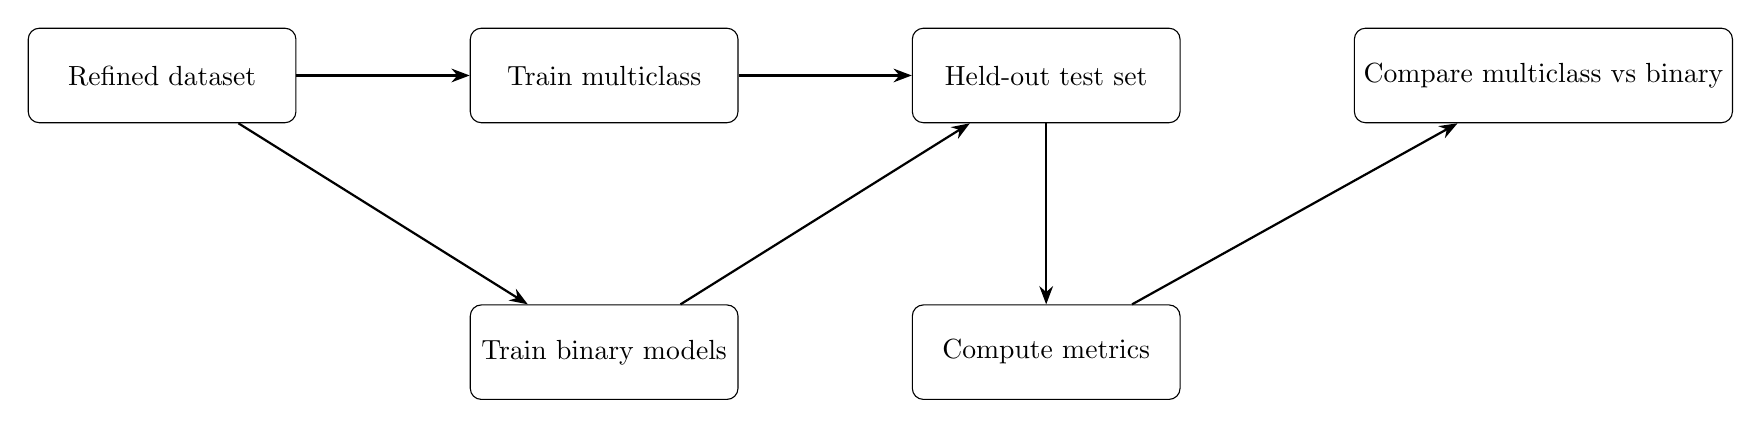
\begin{tikzpicture}[node distance=2.3cm and 2.2cm, box/.style={draw, rounded corners, align=center, minimum width=3.4cm, minimum height=1.2cm}, arrow/.style={->, >=Stealth, thick}]
\node[box](a){Refined dataset};
\node[box,right=of a](b){Train multiclass};
\node[box,below=of b](c){Train binary models};
\node[box,right=of b](d){Held-out test set};
\node[box,below=of d](e){Compute metrics};
\node[box,right=of d](f){Compare multiclass vs binary};
\draw[arrow] (a)--(b);
\draw[arrow] (a)--(c);
\draw[arrow] (b)--(d);
\draw[arrow] (c)--(d);
\draw[arrow] (d)--(e);
\draw[arrow] (e)--(f);
\end{tikzpicture}
\caption{Experimental comparison workflow for future dataset refinement and evaluation.}
\label{fig:comparison-workflow}
\end{figure}

\section{Future Work}
The following areas are relevant as future work for the project, but they are not currently implemented capabilities. They include:
\begin{itemize}[leftmargin=1.5em]
    \item Temporal or video-based modeling using sequential frames or clips.
    \item Tracking and motion-based event reasoning across time.
    \item Better CNN architectures such as deeper residual networks or transfer learning.
    \item Object detection approaches for event-localization tasks.
    \item Temporal aggregation across multiple frames for confidence stabilization.
    \item Confidence calibration and threshold tuning for real-world deployment.
    \item Alert verification and human-in-the-loop review.
    \item Deployment optimization for embedded or edge devices.
\end{itemize}
These remain future extensions rather than current system features.

\section{Conclusion}
The repository implements a functional prototype for surveillance-event classification using a simple Flask-based interface, OpenCV camera streaming, and TensorFlow/Keras CNNs. The system currently contains one multiclass model and three binary event models, all using the same basic CNN architecture and a frame-by-frame preprocessing pipeline. The most defensible academic description of the current project is that it is an experimental comparison between multiclass and binary image classification approaches for surveillance events. The repository clearly indicates several limitations, including small and uneven dataset coverage, potential frame similarity, lack of a formal held-out test set, and the absence of explicit temporal modeling. For these reasons, the project should be presented as an exploratory prototype with baseline or preliminary insights rather than as a production-ready or validated detection system.

\section{References}
\begin{thebibliography}{99}

\bibitem{krizhevsky2012}
A. Krizhevsky, I. Sutskever, and G. E. Hinton, \emph{ImageNet Classification with Deep Convolutional Neural Networks}, Advances in Neural Information Processing Systems (NeurIPS), 2012. \url{https://papers.nips.cc/paper/4824-imagenet-classification-with-deep-convolutional-neural-networks}

\bibitem{simonyan2015}
K. Simonyan and A. Zisserman, \emph{Very Deep Convolutional Networks for Large-Scale Image Recognition}, International Conference on Learning Representations (ICLR), 2015. \url{https://arxiv.org/abs/1409.1556}

\bibitem{he2016}
K. He, X. Zhang, S. Ren, and J. Sun, \emph{Deep Residual Learning for Image Recognition}, IEEE Conference on Computer Vision and Pattern Recognition (CVPR), 2016. \url{https://openaccess.thecvf.com/content_cvpr_2016/html/He_Deep_Residual_Learning_CVPR_2016_paper.html}

\bibitem{redmon2016}
J. Redmon, S. Divvala, R. Girshick, and A. Farhadi, \emph{You Only Look Once: Unified, Real-Time Object Detection}, IEEE Conference on Computer Vision and Pattern Recognition (CVPR), 2016. \url{https://www.cv-foundation.org/openaccess/content_cvpr_2016/html/Redmon_You_Only_Look_CVPR_2016_paper.html}

\bibitem{carreira2017}
J. Carreira and A. Zisserman, \emph{Quo Vadis, Action Recognition? A New Model and the Kinetics Dataset}, IEEE Conference on Computer Vision and Pattern Recognition (CVPR), 2017. \url{https://openaccess.thecvf.com/content_cvpr_2017/html/Carreira_Quo_Vadis_Action_CVPR_2017_paper.html}

\bibitem{wang2016}
L. Wang, Y. Xiong, Z. Wang, Y. Qiao, D. Lin, X. Tang, and L. Van Gool, \emph{Temporal Segment Networks: Towards Good Practices for Deep Action Recognition}, European Conference on Computer Vision (ECCV), 2016. \url{https://link.springer.com/chapter/10.1007/978-3-319-46484-8_2}

\end{thebibliography}

\end{document}
